\chapter{Evaluation methodology and results}\label{chap:evaluation}

This chapter reports the empirical part of the thesis. Section~\ref{sec:setup} describes the evaluation protocol: the datasets, the transaction-cost model, the anchored walk-forward procedure, the baselines, the risk-adjusted metrics, the regime labelling, the volatility-matched comparison, the cost-sensitivity sweep, and the bootstrap tests. Sections~\ref{sec:results} and~\ref{sec:robustness} report the results on the WIG20 panel and the robustness checks together with the external validation on the FTSE~100. Section~\ref{sec:discussion} interprets the evidence against the three hypotheses of Section~\ref{sec:hypotheses}, and Section~\ref{sec:evaluation_summary} closes the chapter.

The protocol described here is the element of the work that addresses the four methodological weaknesses identified in Chapter~\ref{sec:related_work}, and the stage that the template calls testing and verification of results: every headline number is produced on data that was never used to select a parameter, net of realistic frictions, accompanied by confidence intervals, and stress-tested against ablations, weight perturbations, cost grids, and a second market.

\section{Experimental setup}\label{sec:setup}

\subsection{Dataset}\label{subsec:dataset}

Daily OHLCV panels for both experiments come from the public repository Stooq \cite{stooq}. Within a given market the ensemble, the index buy-and-hold benchmark and the machine-learning baselines all trade one fixed roster of constituents, and any incomplete row is dropped from the symbol it belongs to.

The primary panel holds the WIG20 index together with nineteen of its constituent stocks on the Warsaw Stock Exchange. \.{Z}abka Group SA. is left out, its listing date of $2024/10/17$ being far more recent than that of the remaining constituents. Coverage runs from $2021/05/26$ to $2026/03/31$, approximately $1{,}220$ trading days, with all values denominated in PLN.

For external validation the panel consists of \FtseNsymbols{} liquid FTSE~100 constituents plus the FTSE~100 index itself on the London Stock Exchange, spanning the same calendar window and denominated in GBP. Both markets receive an identical anchored split, training up to $2024/06/30$ and testing from $2024/07/01$ through $2026/03/31$. Nothing changes in the agents, the hyperparameters or the evaluation procedures; what differs is confined to the price panels, the index series and the transaction-cost calibration (Sections~\ref{subsec:costs} and~\ref{subsec:ftse}). Section~\ref{sec:data_pipeline} describes how both panels were prepared.

\subsection{Transaction-cost model}\label{subsec:costs}

Every backtest charges a proportional commission of $39$ basis points (bps) of notional on each trade and applies one-way slippage of $5$ bps to the executed price, both figures sitting in the range that Polish retail brokerages typically charge on WSE-listed equities. Commission leaves the cash balance on entry and again on exit. Slippage moves the effective buy price up and the effective sell price down by the stated amount. Realised profit or loss is therefore reported after the commissions on both legs and after round-trip slippage.

That calibration errs on the conservative side for a retail investor and cuts substantially into the headline gross return of any high-turnover configuration, which is precisely the methodological concern raised in the literature on backtest reliability \cite{bailey2014}. Section~\ref{subsec:cost_sensitivity} reports a full sensitivity sweep over commission and slippage.

\subsection{Walk-forward protocol}\label{subsec:walkforward}

An anchored walk-forward protocol governs the evaluation. The full period divides into a training window running from $2021/05/26$ to $2024/06/30$ and a held-out test window running from $2024/07/01$ to $2026/03/31$. Within the training window a grid search covers the decision-agent parameters
\begin{equation}
\begin{aligned}
\mathrm{mode} &\in \{\text{passive}, \text{balanced}, \text{aggressive}\}, \\
c_{\min} &\in \{0, 0.05, 0.10, \ldots, 0.30\},
\end{aligned}
\label{eq:wf_grid}
\end{equation}
whose in-sample total return proves greatest, and that configuration then goes to the test window untouched. Indicator hyperparameters never enter the grid and stay fixed from beginning to end. Holding the degrees of freedom this low matches the way most of the cited literature treats technical-analysis rules.

Retaining total return as the selection objective is deliberate, notwithstanding that the strategy is judged mainly on risk-adjusted metrics, and the reason is statistical rather than conceptual. Ranking $21$ configurations on a low-dimensional grid calls for a simple criterion of low variance, which in-sample total return supplies. Ratio statistics such as the Sharpe ratio do not: on samples of this length they carry substantial estimation error \cite{lo2002}, and they degenerate outright for configurations that trade rarely. Since the \emph{passive} mode places no trades at any threshold (Table~\ref{tab:grid_train}), the in-sample Sharpe ratio it yields is undefined rather than simply poor, which would leave any risk-adjusted objective breaking such ties arbitrarily. Section~\ref{subsec:objective} confirms that nothing rests on the choice, re-running the selection under Sharpe-ratio and Calmar-ratio objectives over the identical grid and finding the selected configuration, and with it every out-of-sample number in this thesis, unchanged on both markets.

A three-fold anchored expanding walk-forward is reported as an additional robustness check. Each fold $k \in \{1, 2, 3\}$ takes as its test slice one of three roughly equal chronological pieces of the held-out window, and trains from $2021/05/26$ up to the day preceding that slice. Every fold receives its own fresh grid search, and its winning configuration is evaluated on its own test slice. The point of the exercise is to demonstrate that the headline configuration owes nothing to one particular split.

Algorithm~\ref{alg:wf} states the full protocol as pseudocode. Its defining feature is that signals are computed once, outside every grid-search and ablation loop. Separating signal computation from the decision-agent grid search in this way cuts end-to-end runtime by better than an order of magnitude, and it renders the sweep in Section~\ref{subsec:costsweep} inexpensive, since altering a cost obliges no agent signal to be recomputed.

\begin{algorithm}[!htbp]
\caption{Anchored walk-forward with precomputed signals}
\label{alg:wf}
\begin{algorithmic}[1]
\STATE \textbf{Input:} prices $P$; agent set $\mathcal{A}$; modes $\mathcal{M}$; thresholds $\mathcal{C}$; train/test split $(T_\text{tr}, T_\text{te})$; costs $(\gamma, s)$.
\STATE \textbf{Output:} selected $(m^\star, c^\star)$; test-window metrics.
\STATE $S \gets \mathtt{PrecomputeSignals}(P, \mathcal{A})$ \COMMENT{all dates, all symbols}
\STATE best $\gets -\infty$
\FORALL{$m \in \mathcal{M}$, $c \in \mathcal{C}$}
  \STATE $E_\text{tr} \gets \mathtt{Backtest}(S, T_\text{tr}, m, c, \gamma, s)$
  \STATE $r \gets \mathtt{TotalReturn}(E_\text{tr})$
  \IF{$r > \text{best}$}
    \STATE best $\gets r$; $(m^\star, c^\star) \gets (m, c)$
  \ENDIF
\ENDFOR
\STATE $E_\text{te} \gets \mathtt{Backtest}(S, T_\text{te}, m^\star, c^\star, \gamma, s)$
\RETURN $(m^\star, c^\star)$, $\mathtt{Metrics}(E_\text{te})$
\end{algorithmic}
\end{algorithm}

\subsection{Baselines}\label{subsec:baselines}

Baselines fall into three families. \emph{Index buy-and-hold} comes first: the initial cash buys the WIG20 index on the opening date of the test window and the position is held to the end of it, with the FTSE~100 index substituted under the same rule for the replication. Evaluations of trading strategies conventionally adopt buy-and-hold in this role \cite{dichtl2020}.

The second family consists of \emph{single-agent} runs, in which the decision agent is fed by one signal agent alone, giving five baselines, one for each indicator. Five \emph{leave-one-agent-out} configurations accompany them, each withdrawing a single agent from the otherwise complete ensemble. The third family holds the two \emph{machine-learning baselines} that Section~\ref{subsec:lstm} describes.

On each market every baseline is measured over the same test window, charged the market-specific transaction costs of Sections~\ref{subsec:costs} and~\ref{subsec:ftse}, and run at the decision-agent configuration that the walk-forward protocol selected. Two exceptions apply: buy-and-hold carries no decision-agent parameters at all, and the machine-learning baselines put a learned classifier where the decision agent would otherwise sit.

\subsection{Machine-learning baselines}\label{subsec:lstm}

A directional LSTM classifier after the manner of \cite{fischerkrauss2018} supplies a contemporary learning-based reference point. Per symbol it reads a rolling window of causal daily features drawn from the same price history the agents see, namely multi-horizon returns, realised volatility, and normalised versions of the RSI, ROC, MACD-histogram, Bollinger \%b and moving-average-spread indicators, and from these predicts the probability that the return $h$ days ahead is positive. Architecturally it is one LSTM layer followed by dropout and a linear output unit, trained under binary cross-entropy with the Adam optimiser.

Fairness of the comparison requires that every model-selection decision be taken strictly in sample, and it is. The prediction horizon $h$, the operating threshold and the early-stopping point are all chosen on an internal validation slice cut chronologically out of the training window, and no tuning ever touches the held-out test window. Standardisation statistics for the features are estimated on the training window alone, which leaves the procedure free of look-ahead.

Converting per-symbol probabilities into long or flat positions goes through a symmetric no-trade band about $0.5$. Anything above $0.5 + \delta$ opens a long position or keeps one open, anything below $0.5 - \delta$ closes it, and probabilities falling between the two leave the current position as it stands. The arrangement imitates the hold behaviour of the decision agent and heads off the excessive turnover that re-predicting daily would otherwise generate. In-sample selection settles on a horizon of $h = \LSTMhorizon$ days and a band of $\delta = \LSTMband$ on both markets. The long and flat signals that result run through the same portfolio simulator at identical costs and position sizing, so that whatever difference emerges belongs to the decision rule and not to the accounting.

Second among the machine-learning baselines is a gradient-boosted-trees (GBM) directional classifier \cite{friedman2001}, built on LightGBM \cite{ke2017lightgbm}. Large-scale empirical comparisons place gradient-boosted trees consistently among the strongest learners available for tabular financial features \cite{krauss2017,gukellyxiu2020}, which makes them a natural complement to the recurrent LSTM and structurally quite unlike it.

The GBM reads, for every symbol and day, the same causal daily features the LSTM reads, extended by lagged copies of each feature out to $20$ trading days, which gives the flat feature vector a temporal context comparable to the LSTM lookback window. Training pools the feature rows across symbols, divides them chronologically into training and validation slices, stops early on validation log-loss, and averages three models grown from different seeds. As with the LSTM, the prediction horizon and the no-trade band are fixed strictly in sample, here by the net-of-cost Sharpe ratio of a portfolio simulation on the validation slice, and the long and flat signals produced pass through the same portfolio simulator under identical costs. In-sample selection yields $h = \GBMhorizon$ with $\delta = \GBMband$ on WIG20, and $h = \FtseGBMhorizon$ with $\delta = \FtseGBMband$ on the FTSE~100.

\subsection{Risk-adjusted metrics}\label{subsec:metrics}

Metrics are computed from the equity curve and from the list of closed trades, as follows. \textbf{Total return} gives the percentage change in portfolio value between the first and the last date of the evaluation window. \textbf{CAGR} (compound annual growth rate) annualises that return over the same window. \textbf{Max drawdown} takes the largest peak-to-trough decline and reports it as a negative fraction. \textbf{Sharpe ratio} \cite{sharpe1966} divides annualised excess return by standard deviation, annualising with a factor of $\sqrt{252}$ and assuming a risk-free rate of zero.

\textbf{Sortino ratio} \cite{sortino1994} substitutes downside deviation into that denominator, so that only below-target returns are penalised:
\begin{equation}
\mathrm{Sortino} = \frac{\sqrt{252}\,\bar{r}}{\sqrt{\tfrac{1}{N}\sum_{t=1}^{N}\min(r_t, 0)^2}},
\label{eq:sortino}
\end{equation}
with $\bar{r}$ the mean daily return and the denominator the downside deviation. \textbf{Calmar ratio} \cite{young1991} divides CAGR by the absolute value of the maximum drawdown. \textbf{Ulcer Index} \cite{martin1989} takes in the whole drawdown path rather than its extremum:
\begin{equation}
\mathrm{UI} = 100 \cdot \sqrt{\tfrac{1}{N}\sum_{t=1}^{N} \mathrm{dd}_t^{\,2}},
\label{eq:ulcer}
\end{equation}
in which $\mathrm{dd}_t$ denotes the running drawdown of the equity curve at date $t$. \textbf{Martin ratio} \cite{martin1989} divides the annualised excess return by the Ulcer Index.

Prolonged drawdowns register more strongly on the Ulcer and Martin statistics than on the peak-to-trough maximum, which is why they serve here as tie-breakers between strategies whose peak drawdowns are alike but whose drawdown profiles are not. \textbf{Number of trades} counts the closed trades, and \textbf{win rate} gives the fraction of them that realised a positive profit.

\subsection{Market-regime labelling}\label{subsec:regimes}

Comparing the ensemble with buy-and-hold on pooled aggregates alone would conceal a good deal, so every trading day of the test window is assigned to one of three regimes, \emph{bull}, \emph{correction} or \emph{sideways}. Nothing beyond information available from the WIG20 index itself up to date $t$ enters the assignment, which keeps it clear of future prices.

Write $\mathrm{high}_t$ for the rolling $252$-day maximum of the WIG20 closing price at $t$, and $\mathrm{ret}_t$ for the price relative $\mathrm{close}_t / \mathrm{high}_t$. A \emph{correction} day is one where $\mathrm{ret}_t < 1 - 0.10$, meaning the index sits at least ten percent under its trailing one-year high. A \emph{bull} day is one where $\mathrm{ret}_t \geq 1 - 0.05$, meaning the index lies within five percent of that high, and where the $50$-day SMA of the WIG20 index stands above its $200$-day SMA. Whatever satisfies neither condition is \emph{sideways}.

Both thresholds are standard in the practitioner literature on market regimes, and neither was tuned on the training data. Applied to the test window, the labelling returns \RegBullShare{} bull days, \RegCorrectionShare{} correction days and \RegSidewaysShare{} sideways days (Table~\ref{tab:regime}), so that all three regimes are represented, and the ensemble faces each one.

\subsection{Volatility-matched comparison}\label{subsec:volmatch}

What follows is an analytical normalisation rather than a directly implementable trading result, and its object is to bring the ensemble and the benchmark onto one risk budget so that their returns may be compared on equal terms. The intuition is straightforward. Spending many days out of the market leaves the ensemble running at lower volatility than a benchmark that is always fully invested, so a bare comparison of cumulative returns penalises it for the risk it declined to take. Removing that confound means multiplying the ensemble returns by a single constant chosen to equate the ex-ante volatilities of strategy and benchmark, and comparing the two equity curves thereafter.

The formal construction begins from a standard criticism of the Sharpe ratio, that its scale invariance measures return per unit of risk while saying nothing about how much risk is being run \cite{harvey2016}. Two strategies may each post a Sharpe ratio of $1.0$ and yet differ in cumulative return if one realises $10\%$ annualised volatility and the other $20\%$, for no reason beyond the second taking more risk.

The remedy is to scale the equity curve of the ensemble, ex ante, onto the realised training-window volatility of buy-and-hold WIG20. That target is the annualised standard deviation of WIG20 daily returns over the training window, $\sigma^{\text{target}} = \sqrt{252}\, \mathrm{std}(r^{\text{WIG20}}_\text{train}) = \BHOosVol{}$, set against a strategy volatility over the same window of $\sigma^{\text{strat}} = \sqrt{252}\,\mathrm{std}(r^{\text{ensemble}}_\text{train}) = \StrategyTrainVol{}$. Their quotient gives the leverage factor $\lambda = \sigma^{\text{target}} / \sigma^{\text{strat}} = \Leverage{}$, held constant across the test window and applied to the out-of-sample ensemble return. Since $\lambda$ derives entirely from training-window data, the comparison is genuinely ex ante and never consults out-of-sample returns.

Two cautions attach to it. The primary finding remains the unleveraged ensemble, with the volatility-matched figures serving as a counterfactual on risk budget and not as a recommendation to trade with leverage. And the leverage factor required, $\lambda = \Leverage{}$, exceeds what most retail investors on the WSE could realistically obtain or would prudently employ, so these results are best treated as an analytical ceiling on risk-normalised return, well outside what practice would allow. Section~\ref{subsec:volscaled} reports the scaled equity curve together with its metrics.

\subsection{Cost-sensitivity sweep}\label{subsec:costsweep}

Beyond the baseline calibration of $39$ bps commission with $5$ bps slippage, the transaction-cost parameters are swept across a grid
\begin{equation}
\begin{aligned}
\mathrm{commission} &\in \{0, 10, 20, 39, 60, 80, 100\}\;\text{bps}, \\
\mathrm{slippage} &\in \{0, 5, 10, 20\}\;\text{bps},
\end{aligned}
\label{eq:cost_grid}
\end{equation}
with the walk-forward backtest re-run at every point on it. What matters is that the agent signals are computed once and handed to each backtest, so that nothing but the portfolio-level accounting varies across the sweep. The experiment exists to establish what portion of the advantage the ensemble holds over buy-and-hold on the risk axis is owed to the particular cost calibration chosen. Section~\ref{subsec:cost_sensitivity} presents the complete grid.

\subsection{Bootstrap confidence intervals and tests}\label{subsec:bootstrap}

Put intuitively, a bootstrap draws the observed daily returns repeatedly, at random and with replacement, recomputes on each redrawn series whichever metric is in question, and reads off from the spread of the results how far that metric might have moved by chance alone. No assumption that returns follow a normal distribution is required anywhere in the procedure.

Every point estimate of total return and Sharpe ratio carries a $95\%$ percentile bootstrap confidence interval, computed on the vector of daily returns of the equity curve over $10{,}000$ resamples drawn with replacement. Comparisons with the local index buy-and-hold benchmark, with the best single-agent baseline and with the machine-learning baselines of Section~\ref{subsec:lstm} use a paired bootstrap instead: each resample draws one set of dates and applies it to both series, the difference in the statistic of interest is taken, and the one-sided $p$-value gives the proportion of resamples in which that difference is non-positive. A $p$-value under $0.05$ counts as evidence that the strategy dominates the baseline on the test window.

A bootstrap suits this setting because trading-strategy metrics are known to be distributed non-Gaussianly and path-dependently, and prior work has recommended bootstrap methods precisely here \cite{politis1994}. As the literature on trading-strategy evaluation would lead one to expect, these tests are not anticipated to carry the power needed to detect moderate effect sizes over a single test window of just under two years \cite{bailey2014}. The $p$-values are consequently presented beside the point estimates and confidence intervals, and are not leaned on as the sole arbiter of performance.

\section{Results on the WIG20 panel}\label{sec:results}

This section reports the results obtained on the primary panel. It begins with the parameter selection performed on the training window, then reports the headline and risk-adjusted comparisons against buy-and-hold on the held-out window, decomposes them by market regime, and closes with two experiments that examine the internal mechanism of the ensemble: the empirical correlations between agent signals, and an audit of the confidence heuristic.

\subsection{Parameter selection on training data}\label{subsec:grid}

In-sample total return for every pairing of decision-agent mode with minimum confidence is set out in Table~\ref{tab:grid_train}. The \emph{passive} mode seldom reaches its demanding buy and sell thresholds and, at every value of the minimum confidence, executes no trades whatsoever. The \emph{balanced} mode trades in moderation and returns small positive figures at all thresholds. The highest returns overall belong to the \emph{aggressive} mode, whose best training-window pairing, (\emph{aggressive}, $c_{\min} = \BestMinConf{}$), becomes the configuration carried forward to out-of-sample evaluation.

This accords with the familiar observation that on a trend-rich daily dataset a moderate tolerance for signals tends to maximise gross return, though the transaction-cost model of Section~\ref{subsec:costs} takes a noticeable bite out of the net figure.

\begin{table}[!htbp]
\centering
\caption{In-sample total return (train window, $2021$-$2024$) by decision-agent mode and minimum confidence. Higher is better. Selected configuration in bold.}
\label{tab:grid_train}
\begin{tabular}{lccc}
\toprule
\textbf{$c_{\min}$} & \textbf{passive} & \textbf{balanced} & \textbf{aggressive} \\
\midrule
$0.00$ & 0.00 & 0.05 & 0.48 \\
$0.05$ & 0.00 & 0.09 & \textbf{0.55} \\
$0.10$ & 0.00 & 0.09 & 0.49 \\
$0.15$ & 0.00 & 0.11 & 0.40 \\
$0.20$ & 0.00 & 0.23 & 0.28 \\
$0.25$ & 0.00 & 0.16 & 0.25 \\
$0.30$ & 0.00 & 0.28 & 0.23 \\
\bottomrule
\end{tabular}
\end{table}

\subsection{Headline results on held-out data}\label{subsec:headline}

Headline metrics for the selected configuration and for buy-and-hold WIG20, computed on the held-out test window, are collected in Table~\ref{tab:headline}. Every figure is net of the transaction costs specified in Section~\ref{subsec:costs}.

The benchmark wins on gross total return, taking \BHtest{} across \OOSDays{} trading days against \TRtest{} for the ensemble (CI $[\TRtestCIlow, \TRtestCIhigh]$), with a one-sided bootstrap $p$-value of \PvsBH{} on the hypothesis that the ensemble exceeds it.

Shift the comparison onto the risk axis and it inverts. The ensemble records a Sharpe ratio of \Shtest{} (CI $[\ShtestCIlow, \ShtestCIhigh]$) where buy-and-hold records \BHsharpe{}, at a $p$-value of \PvsBHsharpe{}. Maximum drawdown comes in at \MDDtest{} against \MDDbh{}, better than a twofold reduction, and the Calmar ratio at \Calmtest{} against \Calmbh{}, better than twice as large. The two equity curves are plotted in Fig.~\ref{fig:equity_oos}, and Fig.~\ref{fig:drawdown_oos} lays their underwater curves over one another.

\begin{table}[!htbp]
\centering
\caption{Out-of-sample metrics on the held-out test window, net of transaction costs. Brackets give $95\%$ bootstrap confidence intervals.}
\label{tab:headline}
\begin{tabular}{lcc}
\toprule
\textbf{Metric} & \textbf{Multi-agent system} & \textbf{Buy-and-hold WIG20} \\
\midrule
Total return     & $\TRtest$ $[\TRtestCIlow, \TRtestCIhigh]$ & $\BHtest$ \\
CAGR             & $\CAGRtest$ & $\CAGRbh$ \\
Max drawdown     & $\MDDtest$  & $\MDDbh$ \\
Sharpe ratio     & $\Shtest$ $[\ShtestCIlow, \ShtestCIhigh]$ & $\BHsharpe$ \\
Calmar ratio     & $\Calmtest$ & $\Calmbh$ \\
Number of trades & $\Ntrades$  & -- \\
Win rate         & $\WinRate$  & -- \\
\bottomrule
\end{tabular}
\end{table}

\begin{figure}[!htbp]
    \centering
    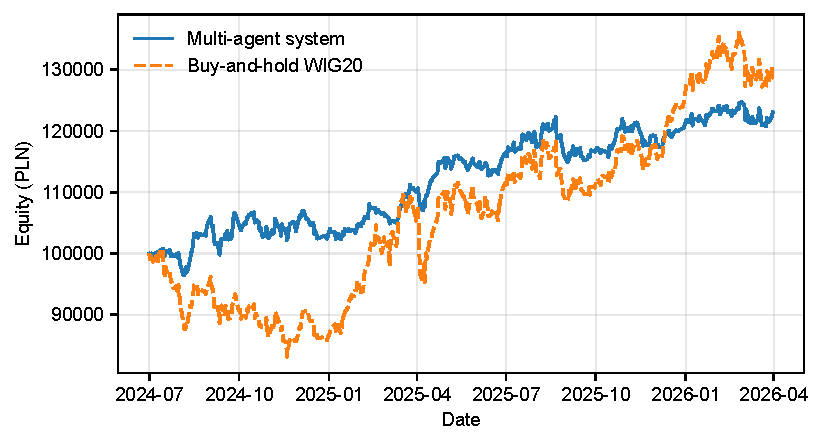
\includegraphics[width=\linewidth]{img/fig_equity_oos.pdf}
    \caption{Equity curves on the held-out test window for the multi-agent system (selected configuration) and for buy-and-hold WIG20. Both series start at the same initial cash and are net of transaction costs.}
    \label{fig:equity_oos}
\end{figure}

\begin{figure}[!htbp]
    \centering
    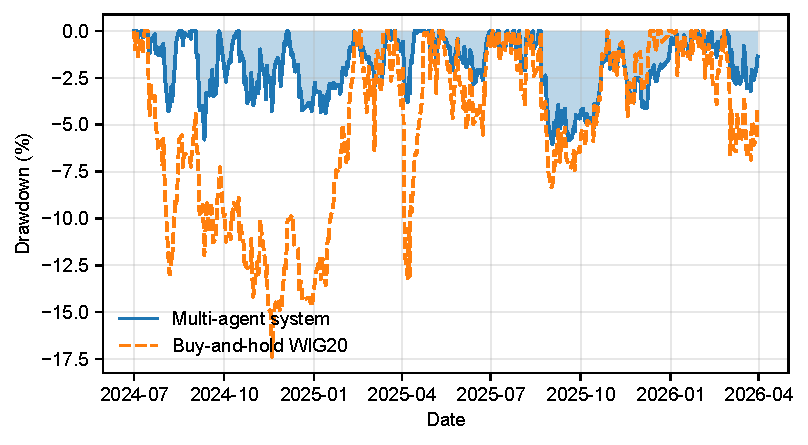
\includegraphics[width=\linewidth]{img/fig_drawdown_oos.pdf}
    \caption{Underwater (drawdown) curves for the ensemble and for buy-and-hold WIG20 on the held-out test window. The drawdowns of the ensemble are both shallower and shorter, which is the central risk-adjusted finding of the thesis.}
    \label{fig:drawdown_oos}
\end{figure}

\subsection{Risk-adjusted comparison}\label{subsec:risk_adjusted}

Extending the set of risk-adjusted measures, as Table~\ref{tab:risk_adjusted} does, only strengthens that inversion. Downside deviation falls from \BHDownDev{} for buy-and-hold to \EnsDownDev{} for the ensemble, a drop of more than forty percent, which carries the Sortino ratio up from \BHSortino{} to \EnsSortino{}.

Because the Ulcer Index registers how deep drawdowns run and how long they persist, rather than only how deep the worst one goes, it separates the two series more sharply still: \EnsUlcer{} for the ensemble against \BHUlcer{} for buy-and-hold, a reduction approaching two-thirds. The Martin ratio moves correspondingly, from \BHMartin{} to \EnsMartin{}, better than a factor of two. Rolling $60$-day Sharpe ratios for both series are plotted in Fig.~\ref{fig:rolling_sharpe}, where the ensemble sits above the benchmark across most of the test window and conspicuously so through the correction subperiods.

\begin{table}[!htbp]
\centering
\caption{Risk-adjusted metrics on the held-out test window, net of transaction costs.}
\label{tab:risk_adjusted}
\begin{tabular}{lcc}
\toprule
\textbf{Metric} & \textbf{Multi-agent system} & \textbf{Buy-and-hold WIG20} \\
\midrule
Sharpe ratio         & $\Shtest$     & $\BHsharpe$ \\
Sortino ratio        & $\EnsSortino$ & $\BHSortino$ \\
Downside deviation   & $\EnsDownDev$ & $\BHDownDev$ \\
Calmar ratio         & $\Calmtest$   & $\Calmbh$ \\
Max drawdown         & $\MDDtest$    & $\MDDbh$ \\
Ulcer Index          & $\EnsUlcer$   & $\BHUlcer$ \\
Martin ratio         & $\EnsMartin$  & $\BHMartin$ \\
\bottomrule
\end{tabular}
\end{table}

\begin{figure}[!htbp]
    \centering
    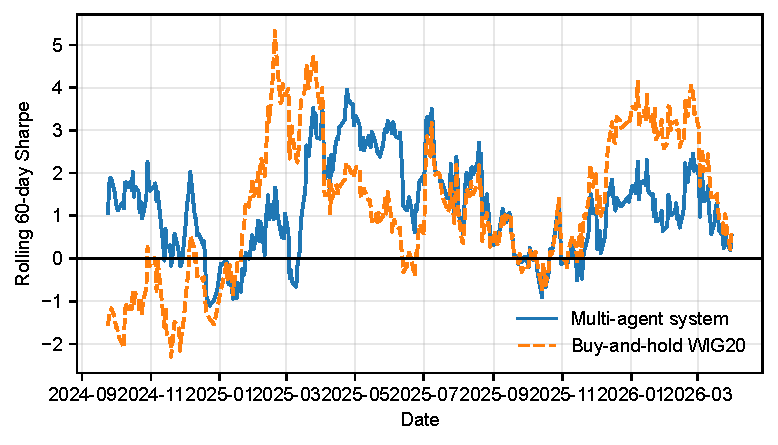
\includegraphics[width=\linewidth]{img/fig_rolling_sharpe.pdf}
    \caption{Rolling $60$-day Sharpe ratio of the ensemble and of buy-and-hold WIG20 on the held-out test window. The rolling Sharpe of the ensemble exceeds buy-and-hold during correction subperiods and is close to it during the bull leg.}
    \label{fig:rolling_sharpe}
\end{figure}

\subsection{Volatility-matched comparison}\label{subsec:volscaled}

Comparing the two series on gross total return is systematically unfair to the ensemble, since they do not run at comparable volatilities. Measured on the training window, the ensemble annualises at $\StrategyTrainVol{}$ and buy-and-hold WIG20 at $\BHOosVol{}$. Equalising the two risk budgets means multiplying its out-of-sample daily returns by the ex-ante leverage factor $\lambda = \Leverage{}$ that Section~\ref{subsec:volmatch} constructs.

Table~\ref{tab:volmatched} collects what results. Matched on volatility, the ensemble returns \VolScaledTR{} where buy-and-hold returns \BHtest{}, an advantage of \VolScaledExcessPP{} percentage points. Sharpe is unmoved at \VolScaledSharpe{}, necessarily so, since ignoring cash reserves makes it scale-invariant in the leverage factor. Sortino comes to \VolScaledSortino{} against \BHSortino{}, and Calmar to \VolScaledCalmar{} against \Calmbh{}. Maximum drawdown under matching is \VolScaledMDD{}, which remains materially below the \MDDbh{} of buy-and-hold notwithstanding the far greater leverage, because the correction-regime drawdown of the ensemble is structurally shallower to begin with (Section~\ref{subsec:regime}).

These figures are analytical instruments rather than trading instructions. Leverage of magnitude $\lambda = \Leverage{}$ lies beyond what a typical retail investor on the WSE can practically obtain, so what Table~\ref{tab:volmatched} offers is a counterfactual on risk budget, not an outcome anyone could realise. The purpose is corrective: measuring a partially invested strategy at its natural volatility against a fully invested benchmark running at roughly twice that volatility understates how much return per unit of risk the strategy actually delivers.

\begin{table}[!htbp]
\centering
\small
\caption{Volatility-matched out-of-sample metrics. The ensemble is scaled, ex ante, to the buy-and-hold volatility measured on the training window (leverage factor $\lambda = \Leverage{}$).}
\label{tab:volmatched}
\begin{tabular}{lccc}
\toprule
\textbf{Metric} & \textbf{Ensemble} & \textbf{Ensemble} & \textbf{Buy-and-hold} \\
                & \textbf{(unleveraged)} & \textbf{(vol-matched)} & \textbf{WIG20} \\
\midrule
Total return     & $\TRtest$     & $\VolScaledTR$      & $\BHtest$ \\
CAGR             & $\CAGRtest$   & $\VolScaledCAGR$    & $\CAGRbh$ \\
Sharpe ratio     & $\Shtest$     & $\VolScaledSharpe$  & $\BHsharpe$ \\
Sortino ratio    & $\EnsSortino$ & $\VolScaledSortino$ & $\BHSortino$ \\
Max drawdown     & $\MDDtest$    & $\VolScaledMDD$     & $\MDDbh$ \\
Calmar ratio     & $\Calmtest$   & $\VolScaledCalmar$  & $\Calmbh$ \\
Ulcer Index      & $\EnsUlcer$   & $\VolScaledUlcer$   & $\BHUlcer$ \\
\bottomrule
\end{tabular}
\end{table}

\subsection{Market-regime decomposition}\label{subsec:regime}

Three markedly different market regimes are blended together in the aggregates of Table~\ref{tab:headline}. Under the labelling of Section~\ref{subsec:regimes} the test window holds \RegBullDays{} bull days ($\RegBullShare{}$ of it), \RegCorrectionDays{} correction days ($\RegCorrectionShare{}$) and \RegSidewaysDays{} sideways days ($\RegSidewaysShare{}$). Table~\ref{tab:regime} separates the total return and the Sharpe ratio of the ensemble and of buy-and-hold WIG20 across those three.

Through the corrections the ensemble gives up $\EnsCorrectionTR{}$ where buy-and-hold gives up $\BHCorrectionTR{}$, a defensive margin of \CorrectionDefencePP{} percentage points. Through the sideways stretches it takes $\EnsSidewaysTR{}$ against $\BHSidewaysTR{}$ for the benchmark, an excess of \SidewaysExcessPP{} percentage points. Through the bull phases the ordering reverses, $\EnsBullTR{}$ against $\BHBullTR{}$, a shortfall of \BullShortfallPP{} percentage points.

That accounting reconciles the aggregate numbers of Table~\ref{tab:headline}. Full exposure through the bull leg lets buy-and-hold collect most of its upside, whereas the ensemble deliberately reduces exposure across the correction and sideways regimes and surrenders part of the bull-regime upside as the price. Where a bull regime dominates a test window, aggregate total return will favour the fully invested benchmark mechanically; give the window a larger correction share and the aggregate comparison would swing to the ensemble.

\begin{table}[!htbp]
\centering
\small
\setlength{\tabcolsep}{4pt}
\caption{Decomposition of the held-out test window into bull, correction, and sideways subperiods. Shares refer to the fraction of trading days in the test window.}
\label{tab:regime}
\begin{tabular}{lrrrrrr}
\toprule
\textbf{Regime} & \textbf{Days} & \textbf{Share} & \textbf{Ens. TR} & \textbf{Ens. Sharpe} & \textbf{B\&H TR} & \textbf{B\&H Sharpe} \\
\midrule
Bull & 230 & 52.9\% & $0.26$ & $2.47$ & $0.63$ & $2.76$ \\
Correction & 93 & 21.4\% & $-0.07$ & $-1.34$ & $-0.20$ & $-2.41$ \\
Sideways & 112 & 25.7\% & $0.05$ & $0.93$ & $-0.00$ & $0.11$ \\
All & 435 & 100.0\% & $0.23$ & $1.06$ & $0.31$ & $0.82$ \\
\bottomrule
\end{tabular}
\end{table}

\subsection{Cost-sensitivity analysis}\label{subsec:cost_sensitivity}

Out-of-sample Sharpe ratios across the cost grid of Section~\ref{subsec:costsweep} are tabulated in Table~\ref{tab:cost_sensitivity}. Charging nothing yields \CostZeroSharpe{}; the baseline calibration of $39$ bps commission with $5$ bps slippage yields \CostBaseSharpe{}; the harshest corner of the grid, $100$ bps commission with $20$ bps slippage, brings it down to \CostWorstSharpe{}. Nowhere on the grid does the ratio fall to the benchmark level, its minimum of \CostMinSharpe{} still exceeding the buy-and-hold Sharpe of \BHsharpe{}.

Total return, computed alongside Sharpe but omitted from the table for brevity, tells the same story qualitatively. At every point on the grid the ensemble trails buy-and-hold on gross total return, and at every point it posts a higher Sharpe ratio, a higher Sortino ratio and a smaller drawdown. The risk-adjusted edge is thus not manufactured by one particular cost calibration, but is a stable property of the strategy across the plausible range of retail brokerage fees.

\begin{table}[!htbp]
\centering
\caption{Cost sensitivity of the out-of-sample Sharpe ratio. Rows are commission in basis points; columns are one-way slippage in basis points.}
\label{tab:cost_sensitivity}
\begin{tabular}{lcccc}
\toprule
\textbf{Commission (bps)} & \textbf{0 bp} & \textbf{5 bp} & \textbf{10 bp} & \textbf{20 bp} \\
\midrule
0 & 1.15 & 1.14 & 1.13 & 1.11 \\
10 & 1.13 & 1.12 & 1.11 & 1.09 \\
20 & 1.11 & 1.10 & 1.09 & 1.07 \\
39 & 1.07 & 1.06 & 1.05 & 1.03 \\
60 & 1.03 & 1.02 & 1.02 & 0.99 \\
80 & 0.99 & 0.99 & 0.98 & 0.96 \\
100 & 0.96 & 0.95 & 0.94 & 0.92 \\
\bottomrule
\end{tabular}
\end{table}

\subsection{Empirical signal correlations}\label{subsec:correlations}

Everything the variance-reduction argument of Section~\ref{sec:forecast_combination} claims depends on the five agents producing signals whose errors are imperfectly correlated. Table~\ref{tab:corr} puts that dependence to the test, giving the pairwise Pearson correlations \cite{pearson1896} of the signed confidence values over all pooled (symbol, date) observations in the training window.

Over \CorrN{} distinct pairs the mean absolute off-diagonal correlation is \CorrMeanAbs{}, bounded by \CorrMin{} at one end (RSI against ROC) and \CorrMax{} at the other (RSI against Bollinger). The momentum family (MACD, ROC) and the mean-reversion family (RSI) correlate negatively, which follows from their reading the same raw price input in opposite directions, and the trend agent (MA trend) comes out close to uncorrelated with everything else, which follows from its much longer horizon.

The same matrix is rendered as a heatmap in Fig.~\ref{fig:corr_matrix}. What these measurements supply is the non-identical-errors assumption of \eqref{eq:combined_variance} in concrete form, and Section~\ref{sec:discussion} draws on them again in explaining why most of the variance reduction comes from the interplay of the momentum and mean-reversion families rather than from the trend agent acting on its own.

\begin{table}[!htbp]
\centering
\caption{Pearson correlations of the pooled (symbol, date) signed confidence values of the five signal agents, computed on the training window. Upper triangle shown.}
\label{tab:corr}
\begin{tabular}{lccccc}
\toprule
 & \textbf{MACD} & \textbf{RSI} & \textbf{ROC} & \textbf{Bollinger} & \textbf{MA trend} \\
\midrule
MACD & \textbf{1.00} & -0.01 & +0.04 & -0.34 & -0.04 \\
RSI &  & \textbf{1.00} & -0.71 & +0.46 & +0.12 \\
ROC &  &  & \textbf{1.00} & -0.55 & -0.12 \\
Bollinger &  &  &  & \textbf{1.00} & +0.09 \\
MA trend &  &  &  &  & \textbf{1.00} \\
\bottomrule
\end{tabular}
\end{table}

\begin{figure}[!htbp]
    \centering
    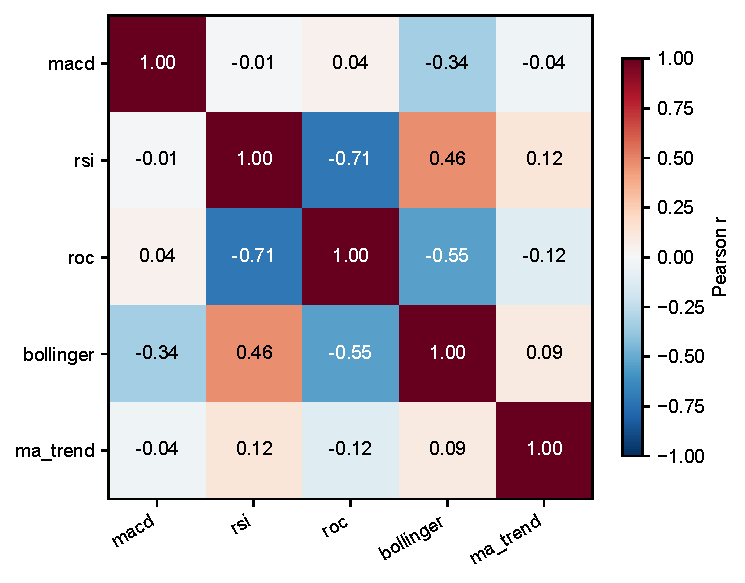
\includegraphics[width=0.85\linewidth]{img/fig_corr_matrix.pdf}
    \caption{Heatmap of the pairwise Pearson correlations of the agent signed-confidence signals on the training window. Blue cells mark negative correlations, red cells mark positive ones. The largest absolute correlations appear in the RSI-ROC and RSI-Bollinger pairs, which is consistent with their shared reliance on overbought and oversold rules.}
    \label{fig:corr_matrix}
\end{figure}

\subsection{Validation of the confidence measure}\label{subsec:confvalid}

The justification offered for the score \eqref{eq:score} in Section~\ref{sec:mapping} treats per-signal confidence as a heuristic stand-in for inverse forecast variance. Were that reading literally true, it would carry an observable consequence: signals issued at higher confidence ought to get the direction right more often than signals issued at lower confidence.

Table~\ref{tab:confvalid} puts that consequence to the test on the training window, so that no test-window information is used. Every active signal, meaning every signal that is not a hold, is pooled per agent across symbols and dates; its directional hit rate is computed against the following day's move; and confidence is then set against correctness twice over, by a Spearman rank correlation \cite{spearman1904} and by weighing the hit rate of the top confidence quintile against that of the bottom, after the manner of the reliability analysis in \cite{murphywinkler1987}. Rank correlation is the right instrument here because correctness takes only two values and the confidence distributions pile up heavily towards zero, which leaves no warrant for assuming linearity. The exercise complements rather than repeats the Pearson correlations of Section~\ref{subsec:correlations} \cite{pearson1896}, which concern the association \emph{between} agents, not that between the confidence of an agent and its own accuracy.

\begin{table}[!htbp]
\centering
\setlength{\tabcolsep}{4pt}
\small
\caption{Confidence validation on the WIG20 training window at the one-day horizon. $\rho$ is the Spearman rank correlation between confidence and directional correctness, with its $p$-value; Hit (Q1) and Hit (Q5) are hit rates in the bottom and top confidence quintiles.}
\label{tab:confvalid}
\begin{tabular}{lrccccc}
\toprule
\textbf{Agent} & \textbf{$n$} & \textbf{Hit rate} & \textbf{$\rho$} & \textbf{$p$} & \textbf{Hit (Q1)} & \textbf{Hit (Q5)} \\
\midrule
MACD & $1{,}405$ & $0.472$ & $+0.002$ & $0.955$ & $0.470$ & $0.484$ \\
RSI & $3{,}847$ & $0.497$ & $-0.035$ & $0.031$ & $0.525$ & $0.497$ \\
ROC & $11{,}155$ & $0.498$ & $+0.016$ & $0.082$ & $0.494$ & $0.520$ \\
Bollinger & $1{,}674$ & $0.483$ & $-0.004$ & $0.867$ & $0.478$ & $0.481$ \\
MA trend & $10{,}982$ & $0.505$ & $-0.004$ & $0.690$ & $0.503$ & $0.500$ \\
Pooled & $29{,}063$ & $0.498$ & $+0.003$ & $0.578$ & $0.493$ & $0.495$ \\
\bottomrule
\end{tabular}
\end{table}

There is no ambiguity in the answer. The confidence values hold no usable information whatever about accuracy at the level of individual signals. Pooling \ConfN{} training-window signals gives a hit rate of \ConfPooledHit{}; the per-agent rank correlations occupy $[\ConfRhoMin{}, \ConfRhoMax{}]$ and not one of them exceeds $|\rho| = \ConfRhoMaxAbs{}$; and the top confidence quintile shows no systematic accuracy advantage over the bottom one.

One entry in Table~\ref{tab:confvalid} is nominally significant (RSI, $p = 0.031$), and its sign is negative, so that greater confidence goes together with marginally \emph{worse} calls. It accounts for well under one percent of the variance in correctness and does not withstand a multiple-testing correction over the ten agent-horizon combinations examined, which makes it evidence against the inverse-variance reading rather than for it. Lengthening the horizon to five days changes nothing (pooled hit rate \ConfPooledHitFive{}), and the FTSE~100 training window returns the same verdict (largest per-agent $|\rho| = \FtseConfRhoMaxAbs{}$, pooled hit rate \FtseConfPooledHit{}).

Two consequences follow. The first is that reading the confidence values as inverse variances is a conceptual analogy and not an empirically calibrated property of the system. Taken one signal at a time and at short horizons, the agents behave close to uninformed forecasters, and the magnitude of the confidence attached does nothing to separate the good calls from the bad. The low tuned threshold ($c_{\min} = \BestMinConf{}$) fits that picture, functioning in practice as a mild noise filter rather than as a precision weight.

The second is that precision-weighted averaging cannot be credited with the risk-adjusted performance recorded in the preceding subsections. Two other things are doing the work: the pooling of signals that correlate weakly or negatively across the methodological families (Table~\ref{tab:corr}), which depresses the variance of the aggregate position whether or not the individual confidence magnitudes are informative, and the regime exposure profile that thresholding the score induces (Table~\ref{tab:regime}). What this finding implies for the theoretical framing of the thesis is taken up in Section~\ref{sec:discussion}.

\section{Robustness checks and external validation}\label{sec:robustness}

The results of Section~\ref{sec:results} rest on one configuration, one weighting scheme, one chronological split, and one market. This section removes each of those supports in turn. It reports the single-agent and leave-one-agent-out baselines, the sensitivity of the results to the family weights, the comparison against the two machine-learning baselines, the significance analysis, the three-fold walk-forward, the sensitivity to the selection objective, and the full replication of the pipeline on the FTSE~100.

\subsection{Single-agent baselines and leave-one-out ablation}\label{subsec:ablation}

Total return and Sharpe ratio for each of the five single-agent runs, alongside those of the full ensemble, appear in Table~\ref{tab:single_agent}. \BestSingleName{} heads the single-agent field at \BestSingleTR{} total return. Testing the ensemble against that best single agent on total return returns a one-sided bootstrap $p$-value of \PvsBestSingle{}. H2 rests principally on these figures.

\begin{table}[!htbp]
\centering
\caption{Single-agent baselines on the test window, with the selected mode and minimum confidence. All numbers net of costs.}
\label{tab:single_agent}
\begin{tabular}{lcc}
\toprule
\textbf{Agent used} & \textbf{Total return} & \textbf{Sharpe ratio} \\
\midrule
MACD only        & $0.15$ & $0.86$ \\
RSI only         & $0.16$ & $1.03$ \\
ROC only         & $0.00$ & $0.13$ \\
Bollinger only   & $0.00$ & $0.00$ \\
MA trend only    & $-0.00$ & $0.03$ \\
Full ensemble    & $\TRtest$ & $\Shtest$ \\
\bottomrule
\end{tabular}
\end{table}

Table~\ref{tab:ablation} records what happens when each signal agent is withdrawn in turn. Every removal registers somewhere in the headline metrics, so no agent is wholly idle, yet in each case the reduced ensemble still leads buy-and-hold WIG20 on point estimates of Sharpe ratio and of maximum drawdown. H3 rests principally on this.

\begin{table}[!htbp]
\centering
\caption{Leave-one-agent-out ablation on the test window. The variant column indicates which agent was removed.}
\label{tab:ablation}
\begin{tabular}{lcc}
\toprule
\textbf{Variant} & \textbf{Total return} & \textbf{Sharpe ratio} \\
\midrule
Full ensemble & $\TRtest$ & $\Shtest$ \\
no MACD        & $0.28$ & $1.28$ \\
no RSI         & $0.23$ & $0.92$ \\
no ROC         & $0.26$ & $1.17$ \\
no Bollinger   & $0.23$ & $1.06$ \\
no MA trend    & $0.19$ & $1.16$ \\
\bottomrule
\end{tabular}
\end{table}

\subsection{Weight sensitivity and alternative weighting schemes}\label{subsec:weights}

Since $w_\kappa$ constitutes the only fixed prior anywhere in the decision layer, how far the headline results lean on it deserves measurement. Throughout this subsection the walk-forward-selected configuration (\BestMode{}, $c_{\min} = \BestMinConf{}$) is held constant and the weights alone are varied, so that whatever moves can be attributed to the weighting scheme and to nothing else.

Three families of alternatives are put on the held-out window. The first perturbs one family weight at a time by $\pm 25\%$ and $\pm 50\%$, yielding \WSPerturbN{} variants. The second abandons the ordering rationale of Section~\ref{subsec:decision} outright, in two ways: weights made equal across the families, and weights reversed so that volatility ranks highest and trend lowest. The third estimates the weights from the training window alone, again in two ways. \emph{Optimised} weights come from an exhaustive grid over all four families, judged by the same in-sample total-return objective the headline protocol uses. \emph{Inverse-variance} weights are set proportional to the reciprocal of the directional error variance of each family, as measured on training-window signal outcomes, which is the classical prescription of \cite{batesgranger1969} made operational. The named schemes are reported for WIG20 in Table~\ref{tab:weights}.

\begin{table}[!htbp]
\centering
\small
\caption{Alternative weighting schemes on the WIG20 test window, with (mode, $c_{\min}$) fixed at the walk-forward selection. Weights are listed as (trend, momentum, mean-reversion, volatility).}
\label{tab:weights}
\begin{tabular}{lcccc}
\toprule
\textbf{Scheme} & \textbf{Weights} & \textbf{TR} & \textbf{Sharpe} & \textbf{MDD} \\
\midrule
Baseline & $(1.3, 1.0, 0.8, 0.5)$ & $\TRtest$ & $\Shtest$ & $\MDDtest$ \\
Equal & $(1.0, 1.0, 1.0, 1.0)$ & $\WSEqualTR$ & $\WSEqualSharpe$ & $\WSEqualMDD$ \\
Inverted & $(0.5, 0.8, 1.0, 1.3)$ & $\WSInvertedTR$ & $\WSInvertedSharpe$ & $\WSInvertedMDD$ \\
Optimised & $(\WSOptWtrend, \WSOptWmom, \WSOptWmr, \WSOptWvol)$ & $\WSOptTR$ & $\WSOptSharpe$ & $\WSOptMDD$ \\
Inv.-variance & $(\WSIvWtrend, \WSIvWmom, \WSIvWmr, \WSIvWvol)$ & $\WSIvTR$ & $\WSIvSharpe$ & $\WSIvMDD$ \\
Buy-and-hold & -- & $\BHtest$ & $\BHsharpe$ & $\MDDbh$ \\
\bottomrule
\end{tabular}
\end{table}

Three conclusions emerge. The first is that the weights are not what carries the risk-adjusted profile. Out-of-sample Sharpe ratios across the \WSPerturbN{} perturbations occupy $[\WSPerturbSharpeMin{}, \WSPerturbSharpeMax{}]$ and total returns occupy $[\WSPerturbTRMin{}, \WSPerturbTRMax{}]$, while just \WSFixedBelowBH{} of the \WSFixedN{} fixed and theory-implied schemes finish beneath the buy-and-hold Sharpe ratio of \BHsharpe{}. Perturbing the volatility weight changes nothing whatsoever in any of its four variants, for the simple reason that the selected configuration leaves the Bollinger agent essentially inactive.

With hindsight the baseline is not the best available configuration: cutting the momentum-family weight moderately would have served this particular window better, which agrees with the ablation result that dropping MACD helps. The two schemes falling under the benchmark Sharpe ratio do forfeit that portion of the risk-adjusted advantage, but even they hold the maximum drawdown well inside the buy-and-hold \MDDbh{}. Drawdown reduction, the central risk-adjusted finding of this thesis, thus outlives every weighting scheme tried, including those where the Sharpe advantage does not.

The second conclusion is that fitting the weights in sample gains little. Grid optimisation returns almost the fixed prior back again, moving only the momentum weight, from $1.0$ to $\WSOptWmom{}$, and its out-of-sample total return of \WSOptTR{} sits roughly two percentage points from the baseline. The FTSE~100 goes further and has the optimised weights \emph{lose} to the fixed prior out of sample (\FtseWSOptTR{} against \FtseTRtest{} on total return). That is the forecast combination puzzle in miniature, with the estimation error in the fitted weights consuming the gains they appeared to offer \cite{smithwallis2009,claeskens2016}.

The third conclusion is that the inverse-variance prescription has nothing to say in this setting. Directional hit rates barely differ between the families (Section~\ref{subsec:confvalid}), so the estimation delivers weights that are nearly equal ($\WSIvWtrend{}$, $\WSIvWmom{}$, $\WSIvWmr{}$, $\WSIvWvol{}$ for trend, momentum, mean reversion and volatility), and performance accordingly matches the equal-weight scheme almost exactly.

Repeating the whole experiment on the FTSE~100 reproduces the qualitative pattern, with perturbation Sharpe ratios spanning $[\FtseWSPerturbSharpeMin{}, \FtseWSPerturbSharpeMax{}]$ and \FtseWSFixedBelowBH{} of \FtseWSFixedN{} fixed schemes under the buy-and-hold Sharpe ratio. Set beside the leave-one-agent-out ablation, these results say that what the ensemble contributes does not depend on the particular weight values chosen, and that the coarse fixed prior holds up against perturbed, reordered, optimised and theory-implied alternatives alike.

\subsection{Comparison with machine-learning baselines}\label{subsec:lstm_results}

Table~\ref{tab:lstm} sets the ensemble against the two machine-learning baselines of Section~\ref{subsec:lstm} over the held-out WIG20 window. The LSTM finishes at \LSTMtest{} total return and a Sharpe ratio of \LSTMsharpe{}, where the ensemble reaches \TRtest{} and \Shtest{} and buy-and-hold \BHtest{} and \BHsharpe{}. The ensemble is ahead on total return, on Sharpe ratio and on maximum drawdown (\MDDtest{} against \LSTMmdd{}), and it gets there on a far smaller number of trades (\Ntrades{} against \LSTMtrades{}). One-sided paired bootstrap $p$-values for the ensemble exceeding the LSTM come to \PensVsLSTM{} on total return and \PensVsLSTMsharpe{} on Sharpe ratio, so, just as in the buy-and-hold comparison, a sizable point-estimate advantage still falls short of the conventional $p < 0.05$ threshold on a single test window.

The GBM baseline behaves much the same way, returning \GBMtest{} at a Sharpe ratio of \GBMsharpe{} across \GBMtrades{} closed trades. Statistically its equity path cannot be separated from that of the LSTM (paired one-sided $p = \PGBMvsLSTM{}$ on total return), and the ensemble again leads on total return, on Sharpe ratio and on Calmar ratio (one-sided $p = \PensVsGBM{}$ on total return and $p = \PensVsGBMsharpe{}$ on Sharpe ratio).

Maximum drawdown is the one measure on which the GBM comes out in front (\GBMmdd{} against \MDDtest{}), and what lies behind that number is a nearly flat equity curve rather than superior risk control. Very little risk is taken and correspondingly little is earned, which the Calmar ratio duly registers (\GBMcalmar{} against \Calmtest{}). That two learners as structurally unlike as a recurrent network and a boosted-tree ensemble, each tuned wholly in sample beneath one protocol, should converge on out-of-sample results this modest reinforces the earlier reading. Flexible learners find little to exploit in the WIG20 test window, while the transparent forecast-combination ensemble stays competitive without being trained at all, which accords with the wider finding that simple, well-regularised combinations hold their own against more flexible learners on noisy financial series \cite{clemen1989,timmermann2006}.

\begin{table}[!htbp]
\centering
\small
\caption{Comparison of the ensemble, the LSTM and GBM directional baselines, and buy-and-hold on the held-out WIG20 test window, net of transaction costs.}
\label{tab:lstm}
\begin{tabular}{lcccc}
\toprule
\textbf{Metric} & \textbf{Multi-agent} & \textbf{LSTM} & \textbf{GBM} & \textbf{Buy-and-hold} \\
\midrule
Total return     & $\TRtest$   & $\LSTMtest$   & $\GBMtest$   & $\BHtest$ \\
Sharpe ratio     & $\Shtest$   & $\LSTMsharpe$ & $\GBMsharpe$ & $\BHsharpe$ \\
Max drawdown     & $\MDDtest$  & $\LSTMmdd$    & $\GBMmdd$    & $\MDDbh$ \\
Calmar ratio     & $\Calmtest$ & $\LSTMcalmar$ & $\GBMcalmar$ & $\Calmbh$ \\
Number of trades & $\Ntrades$  & $\LSTMtrades$ & $\GBMtrades$ & -- \\
\bottomrule
\end{tabular}
\end{table}

\subsection{Statistical significance}\label{subsec:significance}

Two kinds of evidence are attached to the point estimates by the bootstrap. The first is interval evidence. Percentile confidence intervals at the $95\%$ level express the sampling uncertainty that a test window of \OOSDays{} trading days necessarily carries, and for the ensemble they run $[\TRtestCIlow, \TRtestCIhigh]$ on total return and $[\ShtestCIlow, \ShtestCIhigh]$ on Sharpe ratio. Both buy-and-hold point estimates, \BHtest{} on total return and \BHsharpe{} on Sharpe ratio, fall strictly inside those intervals, which is the statistical way of saying that the hypothesis of a common underlying mean return and Sharpe ratio cannot be rejected on this window.

The second is test evidence. Paired against buy-and-hold, the one-sided $p$-values come to \PvsBH{} on total return and \PvsBHsharpe{} on Sharpe ratio, and neither clears the conventional $p < 0.05$ threshold.

Two readings are available. On the risk axis, meaning drawdown, Sortino, Ulcer and Martin, the test-window point estimates favour the ensemble consistently, by margins that are economically large and hold up reasonably well across the ablation and cost grids. Yet rejecting a null of equal mean performance on a single window of under two years is difficult, because trading-strategy return distributions are heavy-tailed and path-dependent \cite{politis1994,bailey2014}. Standard practice in this literature is therefore followed: point estimates, confidence intervals and $p$-values are presented together, and no $p$-value is treated as the sole arbiter. That the buy-and-hold estimates sit inside the bootstrap intervals of the ensemble supports treating the two series as statistically indistinguishable on gross total return, while the large and repeated gap on drawdown-based and downside-based metrics supports the risk-aware reading of what the ensemble contributes (Section~\ref{sec:discussion}).

Two points bear emphasis if these numbers are to be read correctly. One concerns how wide the intervals are. Total return at $[\TRtestCIlow, \TRtestCIhigh]$ and Sharpe at $[\ShtestCIlow, \ShtestCIhigh]$ come out broad because \OOSDays{} trading days furnish relatively few independent realisations of the quantities being estimated, and because serial dependence and heavy tails together inflate the variance of the resampled statistics. At this sample length the paired bootstrap has limited power, and even a genuine moderate edge would frequently fail to register at $p < 0.05$. The non-significant $p$-values are consequently a symptom of a short out-of-sample window, and not positive evidence that the two strategies are equivalent.

The other concerns the gap between practical and statistical significance. What the ensemble achieves on the drawdown-based and downside-based metrics is practically significant, in that the margins are economically large and stable across the ablation, cost and regime analyses, and at the same time not statistically significant, in that no null hypothesis is rejected on this one window. The contribution of the ensemble is framed throughout the thesis accordingly, as consistent and practically meaningful risk reduction, and no claim of statistical dominance over buy-and-hold is advanced anywhere.

\subsection{Walk-forward robustness}\label{subsec:kfold}

Results of the anchored three-fold walk-forward appear in Table~\ref{tab:kfold}, giving for every fold both the configuration chosen on its training window and the total return achieved on its test slice. That choice holds steady from fold to fold, which says that the headline configuration is not an artefact of one particular chronological split.

\begin{table}[!htbp]
\centering
\caption{Anchored walk-forward with $K = 3$ folds. Selected mode and minimum confidence per fold, plus the test-window total return of each fold.}
\label{tab:kfold}
\begin{tabular}{lccc}
\toprule
\textbf{Fold} & \textbf{Selected mode} & \textbf{$c_{\min}$} & \textbf{Test total return} \\
\midrule
1 & \texttt{aggressive} & $0.05$ & $0.05$ \\
2 & \texttt{aggressive} & $0.05$ & $0.09$ \\
3 & \texttt{aggressive} & $0.10$ & $0.08$ \\
\bottomrule
\end{tabular}
\end{table}

\subsection{Sensitivity to the selection objective}\label{subsec:objective}

Choosing $(m^\star, c^\star)$ by in-sample total return, as the headline protocol does (Section~\ref{subsec:walkforward}), raises an obvious question: would a risk-adjusted objective have chosen differently? The test is to re-rank the very same training-window grid under two risk-adjusted objectives, the Sharpe ratio and the Calmar ratio, and then to evaluate each winner untouched on the held-out window.

It would not. On WIG20 all three objectives converge on (\ObjSharpeMode{}, $c_{\min} = \ObjSharpeMinConf{}$), and the FTSE~100 replication behaves the same way, returning (\FtseObjSharpeMode{}, $c_{\min} = \FtseObjSharpeMinConf{}$) whichever objective is applied. Substituting a risk-adjusted objective for the total-return one therefore leaves every out-of-sample number reported in this thesis unchanged on both markets.

Table~\ref{tab:grid_train} shows why. No \emph{passive} configuration trades at all, and the \emph{balanced} ones trade too seldom to compete on cumulative return or on ratio statistics, which leaves the argmax inside the \emph{aggressive} column under every objective. Such invariance should not be assumed in general, as it may well break on grids with more degrees of freedom or on longer menus of modes. On the present design, though, it confirms that opting for a simple, low-variance selection objective (Section~\ref{subsec:walkforward}) is not load-bearing, which is what the estimation-noise case against ratio objectives on short training samples would predict \cite{lo2002}.

\subsection{External validation on the FTSE 100}\label{subsec:ftse}

Is the risk-aware profile a property of the WSE or of the method? Settling that requires running the whole pipeline again somewhere else, which is what this section does on the FTSE~100 panel of Section~\ref{subsec:dataset}. Only two things change. The price data become British, and the cost model is recalibrated to UK conditions: $5$ bps of proportional commission, $5$ bps of one-way slippage, and a $50$ bps Stamp Duty Reserve Tax levied on purchases alone. That last item makes the FTSE cost environment asymmetric and, for buying, appreciably harsher than the Polish calibration. Nothing else moves at all: the decision-agent grid, the indicator hyperparameters and the whole evaluation procedure stay exactly as they were.

Walk-forward selection lands on the same decision-agent family it chose for WIG20, \texttt{aggressive} mode, and the resulting configuration is measured over \FtseOOSDays{} held-out trading days. Table~\ref{tab:ftse} carries the headline comparison, and its shape will be familiar. Gross total return again favours the benchmark (\FtseTRtest{} against \FtseBHtest{}), while every risk measure again favours the ensemble, with a Sharpe ratio of \FtseSharpe{} against \FtseBHsharpe{}, a maximum drawdown of \FtseMDD{} against \FtseBHmdd{} for a reduction of roughly one half, and a Calmar ratio of \FtseCalmar{} against \FtseBHcalmar{}.

The extended measures repeat the pattern: Sortino at \FtseEnsSortino{} against \FtseBHSortino{}, Ulcer Index at \FtseEnsUlcer{} against \FtseBHUlcer{}, and downside deviation at \FtseEnsDownDev{} against \FtseBHDownDev{}. Exactly one measure reverses, the Martin ratio (\FtseEnsMartin{} against \FtseBHMartin{}), and it does so narrowly. The explanation lies in the composition of the window: a test period this overwhelmingly bullish leaves buy-and-hold with an integrated drawdown so shallow that a ratio built on it is hard to beat.

\begin{table}[!htbp]
\centering
\small
\setlength{\tabcolsep}{4pt}
\caption{External validation on the FTSE 100 held-out test window, net of transaction costs (including the $50$ bps buy-side Stamp Duty Reserve Tax). Brackets give $95\%$ bootstrap confidence intervals.}
\label{tab:ftse}
\begin{tabular}{lcccc}
\toprule
\textbf{Metric} & \textbf{Multi-agent} & \textbf{LSTM} & \textbf{GBM} & \textbf{Buy-and-hold} \\
\midrule
Total return     & $\FtseTRtest$ $[\FtseTRtestCIlow, \FtseTRtestCIhigh]$ & $\FtseLSTMtest$   & $\FtseGBMtest$ & $\FtseBHtest$ \\
CAGR             & $\FtseCAGR$    & --              & -- & $\FtseBHcagr$ \\
Sharpe ratio     & $\FtseSharpe$ $[\FtseSharpeCIlow, \FtseSharpeCIhigh]$ & $\FtseLSTMsharpe$ & $\FtseGBMsharpe$ & $\FtseBHsharpe$ \\
Max drawdown     & $\FtseMDD$     & $\FtseLSTMmdd$  & $\FtseGBMmdd$ & $\FtseBHmdd$ \\
Calmar ratio     & $\FtseCalmar$  & --              & $\FtseGBMcalmar$ & $\FtseBHcalmar$ \\
Sortino ratio    & $\FtseEnsSortino$ & --           & -- & $\FtseBHSortino$ \\
Ulcer Index      & $\FtseEnsUlcer$   & --           & -- & $\FtseBHUlcer$ \\
Number of trades & $\FtseNtrades$ & $\FtseLSTMtrades$ & $\FtseGBMtrades$ & -- \\
\bottomrule
\end{tabular}
\end{table}

Decomposing by regime accounts for the aggregates. Bull days make up $\FtseRegBullShare{}$ of the FTSE window ($\FtseRegBullDays{}$ days out of \FtseOOSDays{}), leaving only $\FtseRegCorrectionDays{}$ correction days and $\FtseRegSidewaysDays{}$ sideways days, so the correction-regime defence responsible for much of the WIG20 result has almost nowhere to act. The sideways carry survives regardless: across those subperiods the ensemble takes \FtseEnsSidewaysTR{} against \FtseBHSidewaysTR{} for buy-and-hold, reproducing the WIG20 pattern. As before, the aggregate return shortfall sits in the bull regime (\FtseEnsBullTR{} against \FtseBHBullTR{}), where being partially invested mechanically loses to being fully invested. Putting the two series on a common ex-ante volatility, by the construction of Section~\ref{subsec:volscaled}, lifts the ensemble to \FtseVolScaledTR{} at a leverage of $\lambda = \FtseLeverage{}$, which is \FtseVolScaledExcessPP{} percentage points clear of buy-and-hold and still at the shallower drawdown (\FtseVolScaledMDD{}).

On statistical power the paired bootstrap repeats the WIG20 story. Buy-and-hold point estimates fall within the ensemble confidence intervals, and the one-sided $p$-values for the ensemble exceeding the benchmark come to \FtsePvsBH{} on total return and \FtsePvsBHsharpe{} on Sharpe ratio, neither of which reaches $p < 0.05$.

On this window the LSTM baseline outscores the ensemble on point estimates, taking \FtseLSTMtest{} against \FtseTRtest{} on gross total return and \FtseLSTMsharpe{} against \FtseSharpe{} on Sharpe ratio. Neither margin attains statistical significance, \FtsePensVsLSTM{} being the one-sided $p$-value on the ensemble exceeding the LSTM in total return. Two observations place the apparent edge in context. It reflects bull-market exposure rather than better risk control, because the LSTM stays invested almost continuously across a window that is $\FtseRegBullShare{}$ bull and therefore harvests more of the upside while accepting a deeper drawdown (\FtseLSTMmdd{} against \FtseMDD{}). And the LSTM cannot be told apart from passive buy-and-hold on this window either (one-sided $p = \FtsePLSTMvsBH{}$), which is what a near-fully-invested strategy tracking its index looks like statistically. The transparent ensemble, by contrast, gives up part of that exposure by design in return for the shallower drawdown recorded above.

The GBM baseline carries the same pattern to its limit. It records the best point estimates anywhere on the window, \FtseGBMtest{} total return and a Sharpe ratio of \FtseGBMsharpe{}, and arrives there by closing no position whatsoever across the \FtseOOSDays{} held-out days, which amounts to a fully invested stance throughout a window that is \FtseRegBullShare{} bull. On total return its margin does reach marginal significance at five percent, \FtsePensVsGBM{} being the one-sided $p$-value on the ensemble exceeding it, though the matching Sharpe-ratio comparison does not (one-sided $p = \FtsePensVsGBMsharpe{}$), and measured against buy-and-hold the advantage stays statistically non-significant (one-sided $p = \FtsePGBMvsBH{}$ on total return). All of which is the signature of a near-fully-invested strategy riding a bull market rather than of superior risk control.

Its maximum drawdown, \FtseGBMmdd{}, runs deeper than the \FtseMDD{} of the ensemble, and so does that of the LSTM, which leaves the qualitative trade-off where it stood. Staying exposed earns the learning-based baselines more of the bull market, and the ensemble spends that upside deliberately, buying drawdown control with it.

The auxiliary analyses transfer to this market as well. Weight sensitivity produces the same qualitative ranking (Section~\ref{subsec:weights}), the walk-forward selection remains invariant to the objective (Section~\ref{subsec:objective}), and the confidence heuristic proves just as uninformative at signal level (Section~\ref{subsec:confvalid}). The FTSE evidence therefore establishes that the central finding of this thesis, a consistent advantage in drawdown and downside risk over passive buy-and-hold bought with a portion of bull-market upside, carries to a second market whose cost structure differs markedly, and is no artefact of the WIG20 sample.

\section{Discussion}\label{sec:discussion}

This section interprets the results reported above. It first traces the path from forecast-combination theory to the empirical evidence, then assesses the three hypotheses in turn, examines how far the findings generalise across markets, explains why a comparison on gross total return understates what the ensemble contributes, and closes with the practical, deployment, and design implications.

\subsection{From forecast-combination theory to empirical evidence}\label{subsec:theory_to_evidence}

The prediction carried by \eqref{eq:combined_variance} is that a pool of forecasters whose errors are less than perfectly correlated incurs generally less error than the best of its members. Whether that prediction has any purchase on the present system is an empirical question about the agent pool, and Section~\ref{subsec:correlations} answered it. Off-diagonal correlations among the signed confidence values run from $\CorrMin{}$ to $\CorrMax{}$ and average $\CorrMeanAbs{}$ in absolute terms (Table~\ref{tab:corr}, Fig.~\ref{fig:corr_matrix}). Negative pairs count for most in the identity, because a negative $\rho_{kj}$ subtracts from the double sum instead of merely adding little to it, and two such pairs stand out: RSI against ROC at $\CorrMin{}$, and Bollinger against ROC at $-0.55$.

Of these the RSI-ROC pair is the most instructive, because its negative sign is not an accident of the sample but a consequence of how the two rules are built. Oversold conditions read as an opportunity to a mean-reversion rule and as a warning to a momentum rule, so RSI and ROC are constructed to take opposite sides of the same evidence. Disagreement of that kind is what the score in \eqref{eq:score} exists to adjudicate, and it does so by weighing the competing confidences under their family priors. Which family prevails shifts with the market: trend carries the score through bull phases, while mean reversion and volatility recover relative influence when the index moves sideways or falls. Table~\ref{tab:regime} records the consequence of that shifting balance, since the ensemble surrenders less than buy-and-hold in corrections and gains more in sideways stretches, which is the profile a variance-minimising pool of heterogeneous forecasters would be expected to produce.

A worked example makes the arithmetic concrete. Take a WIG20 constituent that has run up sharply across the previous ten sessions. ROC, reading nothing but the speed of that move, returns a buy at high confidence. RSI, compressing the same ten sessions into a $14$-day relative strength that has now passed $70$, returns a sell at moderate confidence. MA trend also returns a buy, since the fast SMA sits above the slow one, but at modest confidence, because the gap between the two averages is small measured against the latest close.

With the family weights fixed as in Section~\ref{subsec:decision}, those three readings enter \eqref{eq:score} as $1.0 \cdot c_\text{ROC}$ and $1.3 \cdot c_\text{MA}$ on the positive side against $-0.8 \cdot c_\text{RSI}$ on the negative. The resulting action is settled by the confidences rather than by a vote: let the overbought reading be emphatic enough and the total falls short of the buy threshold, even with two of the three agents asking to go long. That is \eqref{eq:combined_variance} restated in the vocabulary of the decision layer. A disagreement between a momentum rule and a mean-reversion rule keeps the ensemble out of an exposure that either family, left to itself, would have held, and the accumulated effect of such abstentions is the drawdown profile of Fig.~\ref{fig:drawdown_oos}.

Section~\ref{subsec:confvalid} then fixes the limits of the analogy. Since the confidence magnitudes prove to hold no measurable information about whether a signal is right, the reading of \eqref{eq:score} as an inverse-variance weighting survives only as the motivation that shaped the architecture, and not as a property the built system possesses. Forecast-combination theory offers two claims here, and the evidence separates them. The strong claim, that the more reliable forecasters can be identified and weighted up, finds no support. The weak claim, that pooling imperfectly correlated errors shrinks the variance of the combination however the pool is weighted, is what the data bear out.

Section~\ref{subsec:weights} corroborates that separation from the opposite direction. Equal weights, estimated inverse-variance weights and the fixed prior all land in much the same place out of sample, which is what the combination literature leads one to expect when the pooled members are of comparable individual accuracy \cite{clemen1989,smithwallis2009}. The operative content of the theory in this application is therefore error diversity alone, and every claim made in this thesis is scoped accordingly.

\subsection{Evidence for the three hypotheses}\label{subsec:hypotheses_evidence}

H1 asserted that the system would match or exceed buy-and-hold on risk-adjusted grounds even where it lost on gross return, and four sets of results bear on it: Tables~\ref{tab:headline}, \ref{tab:risk_adjusted}, \ref{tab:volmatched} and~\ref{tab:regime}. Their verdict is affirmative on point estimates. The bull-regime shortfall of $\BullShortfallPP{}$ percentage points is by itself more than sufficient to account for the aggregate deficit on gross total return, so the return comparison is settled inside that one regime. On every risk-adjusted measure computed, meanwhile, the ordering runs the other way: Sharpe ($\Shtest{}$ against $\BHsharpe{}$), Sortino ($\EnsSortino{}$ against $\BHSortino{}$), Calmar ($\Calmtest{}$ against $\Calmbh{}$), Ulcer Index ($\EnsUlcer{}$ against $\BHUlcer{}$), Martin ($\EnsMartin{}$ against $\BHMartin{}$) and maximum drawdown ($\MDDtest{}$ against $\MDDbh{}$).

Equalising the two risk budgets closes the return gap as well. On the volatility-matched basis the ensemble finishes $\VolScaledExcessPP{}$ percentage points ahead of buy-and-hold while still drawing down materially less. Every one of these margins is a point estimate, and Section~\ref{subsec:significance} shows that none attains conventional significance on a single sub-two-year window, so they are read here as consistent and economically meaningful rather than as demonstrated dominance. Section~\ref{subsec:ftse} recovers the same qualitative pattern across \FtseOOSDays{} held-out trading days under UK-specific costs, which speaks to external validity even though H1 was formally posed against WIG20 alone. All of this sits comfortably with the variance-reduction prediction of forecast-combination theory: combining heterogeneous directional forecasts damps the variance of the resulting equity curve, and the damping is visible in the volatility and in the drawdown path alike.

H2 fares similarly. Against the strongest of the five single-agent runs, \BestSingleName{} at $\BestSingleTR$, the full ensemble returns $\TRtest$, an advantage of more than six percentage points over the test window. The paired bootstrap puts that advantage at $\PvsBestSingle$, short of the $p < 0.05$ mark, which is unsurprising given how hard Sharpe-like statistics are to establish over windows shorter than $400$ trading days \cite{bailey2014}. Read through the combination argument, the sign of the gap is what matters: a diversified score carries less error variance than any of its constituents, and it converts that into appreciably more total return without a matching increase in drawdown.

H3 receives the firmest support of the three. Deleting any one signal agent leaves the test-window total return inside a narrow band about the full ensemble, and even the weakest leave-one-out variant still finishes above $0.19$ on total return, above $1$ on Sharpe, and above buy-and-hold on Sortino.

Two entries in the ablation warrant comment. Dropping MACD, and with it part of the momentum family, nudges the headline metrics upward, which says that the fixed prior allots momentum more weight than this particular period rewarded. Section~\ref{subsec:weights} reaches the same verdict by a different route, since deliberately reducing the momentum weight also improves the window, and it adds the caveat that fitting the weights in sample does not reliably capture such period-specific adjustments out of sample. The Bollinger agent is the opposite case: under the selected configuration it opens very few trades at all, so removing it barely disturbs the ensemble, and it functions on this window as a largely dormant member of the forecast pool.

Together these results establish that no individual agent is load-bearing, which is what forecast-combination theory anticipates so long as two imperfectly correlated forecasters survive in the pool. Section~\ref{subsec:weights} carries the same robustness across from the roster of agents to the weighting itself, since neither perturbing, nor reversing, nor re-estimating the family weights from data overturns the qualitative conclusion.

\subsection{Cross-market generalisation}\label{subsec:crossmarket}

The obvious objection to everything above is that it describes a single sample. Section~\ref{subsec:ftse} answers that objection by rebuilding the study on the FTSE~100, where the constituent set, the currency and the cost structure all differ, the last of these including an asymmetric $50$ bps tax levied on purchases only. The conclusion survives the change intact. Over a bull-dominated window the ensemble again finishes behind passive buy-and-hold on gross total return while posting a better Sharpe ratio (\FtseSharpe{} against \FtseBHsharpe{}), a shallower maximum drawdown (\FtseMDD{} against \FtseBHmdd{}), and better Sortino and Ulcer figures, and it again passes the benchmark on total return once the two series are placed on a common ex-ante risk budget.

Recovering the same trade-off twice, and doing so under an added stamp duty that falls hardest on the more active of the two strategies, argues that the drawdown and downside-risk advantage is structural to forecast combination rather than a coincidence of one exchange. The transfer is nonetheless imperfect. Correction days are almost absent from the FTSE window, which denies the correction-regime defence that does most of the work on WIG20 any room to operate, and the integrated-drawdown advantage thins until the Martin ratio tips marginally to buy-and-hold. That is the regime dependence the adaptive markets hypothesis would lead one to expect \cite{lo2004}: the ensemble earns its keep in the regimes it was built to defend, and a window that is bull almost throughout is the least hospitable setting it could be given.

Three further considerations bound how widely the findings should be read beyond these two exchanges. The first is that technical rules do not pay equally everywhere, and what they pay decays as a market matures. Survey work finds rule profitability concentrated in emerging and thinly traded venues and progressively harder to demonstrate in developed ones once transaction costs and data-snooping corrections are imposed \cite{parkirwin2007}, and earlier evidence across Asian markets ties the same profitability to how developed the market is and how large its trading frictions are \cite{bessembinderchan1995}.

Placed on that spectrum, the two markets studied here behave like moderately mature ones in which chasing a single signal has stopped paying, since every single-agent baseline comes out unprofitable or marginal and neither learned model attains a statistically significant edge, and yet in which a disciplined and diversified risk overlay continues to contribute on the risk axis. It follows that the gross-return comparison should look kinder to the ensemble in less efficient, higher-friction markets, whereas in highly developed ones the risk-control profile is the component that ought to travel.

The second consideration is that what transfers is the structure rather than the numbers. Agent interfaces, the anchored walk-forward procedure, the calibrated cost model and the whole evaluation battery carry over unaltered to any exchange that publishes dependable daily closes, and the FTSE replication needed nothing beyond a fresh data source and a fresh cost model. The calibrations themselves, meaning thresholds, weights, commissions and taxes, have to be re-derived market by market, as the asymmetric UK stamp duty makes plain.

The third is that the contribution is regime-bound. It accrues in corrections and sideways phases, so whatever advantage the ensemble realises on a given market will follow the regime composition of the window it is measured over. Sustained bull regimes reward passive exposure mechanically, as both test windows examined here demonstrate. Charting where the framework does and does not hold across a wider set of developed and emerging indices, as Section~\ref{sec:limitations} proposes, is accordingly the most direct continuation of this study.

\subsection{Why gross total return understates the contribution of the ensemble}\label{subsec:why_gross}

Convention compares a trading strategy with buy-and-hold by setting one gross total return beside another and awarding the verdict to whichever is larger. Applied to the present test window, that convention hands the verdict to the passive benchmark, and it does so while the ensemble is running at under half the benchmark drawdown and ahead of it on the Sharpe, Sortino, Calmar, Ulcer and Martin measures alike.

Three observations indicate that a single gross number is the wrong summary statistic in this setting. The first is that being out of the market is a design feature rather than a failure: the decision-agent thresholds withhold a position until the combined score clears a confidence level, so across a window that is $\RegBullShare{}$ bull, any partially invested strategy trails a fully invested one on gross cumulative return more or less by construction. The second is the volatility-matched result of Section~\ref{subsec:volscaled}, which shows that once the two series are given the same ex-ante risk budget the ensemble returns $\VolScaledExcessPP{}$ percentage points more than buy-and-hold, and still at a smaller absolute drawdown. The third is the regime decomposition of Section~\ref{subsec:regime}, which locates the entire aggregate shortfall inside the bull regime, leaving the ensemble level with or ahead of buy-and-hold on gross return through the correction and sideways regimes.

Taken together, the three reframe what is being compared. The ensemble contributes as a \emph{risk-aware decision support tool}, one that gives up a portion of bull-regime upside in exchange for shallower drawdowns and better risk-adjusted performance across the window as a whole.

\subsection{Connections to the broader empirical literature}\label{subsec:connections}

Three well-established regularities of empirical finance align with the pattern documented in Sections~\ref{sec:results} and~\ref{sec:robustness}.

The first concerns momentum. Time-series and cross-sectional momentum have been shown to be empirically orthogonal, so that portfolios holding both achieve better risk-adjusted results than portfolios holding either \cite{jegadeeshtitman1993,moskowitz2012,asness2013}. What Table~\ref{tab:corr} records between the momentum family (MACD, ROC) and the mean-reversion family (RSI) is that same phenomenon observed one level down, at the signal rather than at the portfolio: the two families fall into disagreement precisely on the occasions when one of them would have been wrong unaided, and the decision-agent score folds the disagreement into a more cautious directional bet than either family would have taken by itself.

The second is the adaptive markets hypothesis \cite{lo2004}, on which no individual trading rule can prevail across every regime, for the reason that the efficiency of a market with respect to any particular rule varies over time. Section~\ref{subsec:regime} bears this out. A trend-weighted ensemble cedes ground through the bull regime, where a passive benchmark mechanically outpaces anything less than fully invested, and recovers it through corrections and sideways periods, where the mean-reversion and volatility agents supply directional information that the trend agent alone would not see.

The third comes from the measurement literature, which has argued for decades that the Sharpe ratio on its own cannot properly rank strategies whose drawdown profiles differ \cite{young1991,sortino1994,martin1989}. The gap between the two advantages measured here makes the argument concrete: on Sharpe the ensemble leads by a factor of $1.3$ (\Shtest{} against \BHsharpe{}), on the Martin ratio by a factor of $2.1$ (\EnsMartin{} against \BHMartin{}). Adjusting for realised volatility and adjusting for the full drawdown path are evidently not the same adjustment, which is why the headline claim of this thesis is stated in terms of Calmar and Ulcer rather than of Sharpe alone.

\subsection{Practical implications for a retail investor}\label{subsec:practical}

Two implications matter for a retail investor working on the WSE with ordinary daily data and typical Polish brokerage terms. The first is the drawdown result. The worst realised loss is cut by better than a factor of two, and the integrated drawdown captured by the Ulcer Index by close to two-thirds. That axis tends to govern how retail portfolios are judged in practice, partly because maximum drawdown carries a direct operational meaning, being the deepest unrealised loss the investor has to sit through, and partly because extended drawdowns are empirically associated with abandoning the plan originally adopted.

The second is durability under costs. Every plausible pairing of commission and slippage in the sweep leaves the risk-adjusted advantage over buy-and-hold intact, the punitive $100$ bps and $20$ bps corner included, which sits well above what WSE retail tariffs currently charge. Neither implication requires leverage, and both are usable in the form of decision-support signals laid over a passive benchmark rather than as a substitute for holding it.

Two operational points follow. One is cadence. Nothing in the five agents or the decision agent consumes anything finer than an end-of-day close, so deploying the system amounts to running the pipeline once the WSE has closed and acting on what it recommends at the open or the close of the following session. That requires no intraday infrastructure, no tick data and no order-book integration, which puts adoption within reach outside the institutional segment.

The other is monitoring. Linearity of the decision-agent score in \eqref{eq:score}, weighted as it is by confidence and by family, means the score can be broken back down into per-agent contributions on any given day and charted next to the equity curve. The investor obtains from this an interpretable record of which agents moved each position, and a straightforward way of noticing structural shifts in the signal distribution, an agent whose confidence collapses for a prolonged stretch being the obvious case, with no retraining involved.

Interpretability of that kind distinguishes a theory-motivated forecast-combination design from end-to-end deep-reinforcement-learning trading systems, which as a rule emit a scalar action carrying no transparent attribution back to the individual input signals.

On the markets examined here that transparency costs very little in performance. The WIG20 comparison puts the ensemble ahead of both learned baselines of Section~\ref{subsec:lstm}, structurally unlike each other though they are, fed identical price history and charged identical costs, across total return and every risk-adjusted ratio, the one exception being the marginally shallower GBM drawdown that follows from its taking almost no risk at all (Section~\ref{subsec:lstm_results}). The FTSE~100 window reverses the point estimates, and the total-return gap of the GBM is marginally significant there, but the learned models reach those figures by staying close to fully invested through a window that is bull almost throughout, which leaves them statistically indistinguishable from passive buy-and-hold and without the drawdown control that motivates the ensemble in the first place (Section~\ref{subsec:ftse}). Full per-signal attribution is therefore retained at no loss of competitiveness on the risk axis against opaque learned models.

\subsection{Deployment and scalability}\label{subsec:deployment}

Whether the system can leave the backtest turns on a handful of practical properties, and on most of them the transparent design is favourably placed.

\emph{Computational cost.} Nothing at decision time iterates. Every signal agent evaluates a closed-form indicator over a rolling window, updated incrementally for each symbol, and the decision agent collapses the per-symbol signals into a single confidence-weighted sum followed by a threshold test, exactly as \eqref{eq:score} states. No training, no gradient computation and no specialised hardware enter the decision path, and one pass over the closing prices of the day on a commodity CPU is enough. The LSTM and GBM baselines of Section~\ref{subsec:lstm} do not share this property, nor do end-to-end deep-reinforcement-learning systems, all of which have to be trained and then retrained periodically.

\emph{Scalability across symbols and markets.} Daily work scales as $O(N_\text{symbols} \times N_\text{agents})$, linear in the size of the traded universe, and it parallelises trivially, since each agent reads the history of one symbol on its own through the shared base-agent interface. Section~\ref{subsec:ftse} supplies concrete evidence of market portability: aiming the whole pipeline at another exchange proved to be a matter of configuration, a new data source and a new cost model, and touched neither the agents nor the decision layer.

\emph{Liquidity.} Only large-capitalisation index constituents are traded, at the daily close, and the selected configuration turns over slowly, so at retail size the resting-order footprint stays small. Price impact, partial fills and order-book dynamics fall outside the model and are treated as a limitation in Section~\ref{sec:limitations}.

\emph{Execution latency.} Signals are produced once the session has closed and acted on in the next one, so delays measured in seconds or minutes are immaterial, and neither co-location nor tick data nor order-book integration is called for. On the spectrum of trading infrastructure this places the design at the opposite end from high-frequency trading.

\emph{Portfolio scalability and the retail-institutional distinction.} Capital scales mechanically under the fractional position-sizing rule, but the assumption that orders fill at the closing price without impact caps the deployable capital against average daily volume, which makes the profile most defensible at retail-to-moderate assets under management. A retail investor can run the system as an end-of-day decision-support overlay on a passive benchmark, with neither leverage nor dedicated infrastructure. An institutional user would find the linear scaling and the market-agnostic interface adequate for wider universes, but would at that point be bound by the need for explicit price-impact modelling and by the analytical-only leverage caveat of Section~\ref{subsec:volscaled}.

\subsection{Design implications}\label{subsec:design_implications}

The experiments carry three implications for the design. The first is that the transparency of the decision-agent score, linear in the agent signals and weighted by confidence and by family, serves theory and practice at once. The contribution each agent makes on a given day is legible directly from the score, and the ablation shows that this attribution agrees with the marginal contribution of that agent to the headline metrics.

The second is that Table~\ref{tab:cost_sensitivity} holds the Sharpe ratio strictly above the passive benchmark at every plausible cost configuration, which indicates that the ensemble is not being kept alive by a favourable cost calibration.

The third is that the selected $(\text{mode}, c_{\min})$ pair holds steady across all three walk-forward folds, which suggests that a plain grid search over a long enough training window suffices, and that heavier parameter-adaptation machinery earns nothing at daily frequency on WIG20.

\section{Chapter summary}\label{sec:evaluation_summary}

The evaluation reported in this chapter was designed to produce results that survive scrutiny rather than results that look impressive. Parameters were selected on a training window and never revisited, every trade was charged realistic commissions and slippage, and every headline figure was accompanied by a bootstrap confidence interval and a paired significance test.

Under that protocol, the finding is consistent and narrow. The ensemble does not beat passive buy-and-hold on gross total return in either test window, and on the WIG20 panel it trails by eight percentage points. It does, however, lead on every risk-adjusted metric considered, halves the maximum drawdown, reduces the integrated drawdown by nearly two-thirds, and overtakes the benchmark on total return once the two series are placed on the same ex-ante risk budget. The regime decomposition locates the source of this profile precisely: the ensemble defends during corrections and carries during sideways phases, and pays for both by under-participating in bull legs.

The robustness checks constrain how much of this can be attributed to chance or to arbitrary design choices. The profile survives the removal of any single agent, perturbation and re-estimation of the family weights, every plausible transaction-cost calibration, a change of the selection objective, a three-fold chronological re-split, and a full replication on a second market with a different cost regime. What it does not survive is the demand for conventional statistical significance on a single sub-two-year window, and that limitation is stated plainly rather than glossed over.

One result deserves emphasis because it cuts against the original design intent. The confidence values that the decision agent uses as weights carry no measurable information about signal-level accuracy. The system works, on the risk axis, but not for the reason its architecture suggests: what operates is the pooling of signals that correlate weakly or negatively across the methodological families, not precision weighting. Chapter~\ref{sec:conclusion} returns to what this implies for the contribution of the thesis and for the work that should follow it.
